% VLDB template version of 2020-08-03 enhances the ACM template, version 1.7.0:
% https://www.acm.org/publications/proceedings-template
% The ACM Latex guide provides further information about the ACM template

\documentclass[sigconf, nonacm]{acmart}

%% The following content must be adapted for the final version
% paper-specific
\newcommand\vldbdoi{XX.XX/XXX.XX}
\newcommand\vldbpages{XXX-XXX}
% issue-specific
\newcommand\vldbvolume{14}
\newcommand\vldbissue{1}
\newcommand\vldbyear{2020}
% should be fine as it is
\newcommand\vldbauthors{\authors}
\newcommand\vldbtitle{\shorttitle} 
% leave empty if no availability url should be set
\newcommand\vldbavailabilityurl{https://doi.org/10.5281/zenodo.10703180}
% whether page numbers should be shown or not, use 'plain' for review versions, 'empty' for camera ready
\newcommand\vldbpagestyle{plain} 

\begin{document}
\title{RepEng Project: An Approach for Schema Extraction of JSON and Extended JSON Document Collections}

%%
%% The "author" command and its associated commands are used to define the authors and their affiliations.

\author{Mohammad Mousavi}
\affiliation{%
  \institution{Universität Passau}
  \city{Passau}
  \country{Germany}
}
\email{mousav03@ads.uni-passau.de}


\maketitle


%%% do not modify the following VLDB block %%
%%% VLDB block start %%%
\ifdefempty{\vldbavailabilityurl}{}{
\vspace{.3cm}
\begingroup\small\noindent\raggedright\textbf{Artifact Availability:}\\
The source code, data, and/or other artifacts have been made available at \url{\vldbavailabilityurl}.
\endgroup
}
%%% VLDB block end %%%

\section{Introduction}

In the scholarly work authored by Frozza et al. ~\cite{frozza2018approach}, the authors address the inherent challenges associated with the schemaless characteristics of JSON documents within NoSQL databases. A common feature of NoSQL databases is that they are schemaless, i.e., they allow the storage of data without prior knowledge of their structure ~\cite{sadalage2012nosql}. However, they argue that the lack of a clearly defined schema does not imply a complete absence of a schema.

The paper by Frozza et al. ~\cite{frozza2018approach} introduces an approach called JSON Schema Discovery, which focuses on generating a unified schema from a set of JSON or Extended JSON documents. While emphasizing NoSQL document-oriented databases due to their widespread use, the approach is designed to generate a JSON Schema for any given collection of JSON documents.

The process involves four steps:
\begin{itemize}
    \item (i) Generating raw schemas for each document.
    \item (ii) Grouping these raw schemas.
    \item (iii) Unifying them.
    \item (iv) Generating a final JSON Schema.
\end{itemize}
An example of the output generated during the execution of JSON Schema Discovery Step 1 is illustrated in Figure~\ref{fig:rawschema}.


\section{Original Experiment Description}

The original experiment conducted by Frozza et al. ~\cite{frozza2018approach} involved the implementation of the JSON Schema Discovery approach on a specific hardware setup. They utilized an ASUS K45VM notebook equipped with an Intel\textsuperscript{R} Core TM i7 3610QM processor running at 2.30 GHz and 8GB of RAM. This setup was employed to execute the experiments related to the quality assessment of the schema generation process.

Frozza et al. ~\cite{frozza2018approach} undertook three experiments to assess the quality of schemas generated through JSON Schema Discovery. These experiments encompassed:

\begin{itemize}
    \item a) Quality of JSON document mapping for JSON Schema.
    \item b) Processing Time Evaluation.
    \item c) Comparison with Related Work.
\end{itemize}

\section{Approach assessment}

In light of Frozza et al.'s ~\cite{frozza2018approach} findings, which are detailed in Table~\ref{table1}, we aim to investigate the reproducibility of their results on our system, a MacBook Air with an Apple M1 processor and 8GB of memory. We seek to reproduce their outcomes, considering that we have access to the exact same datasets used in their study.

The central research question guiding our investigation is: To what extent can the results presented by Frozza et al. ~\cite{frozza2018approach} in Table~\ref{table1} be reproduced on our specified system configuration, given the identical datasets?


\begin{figure}
  \centering
  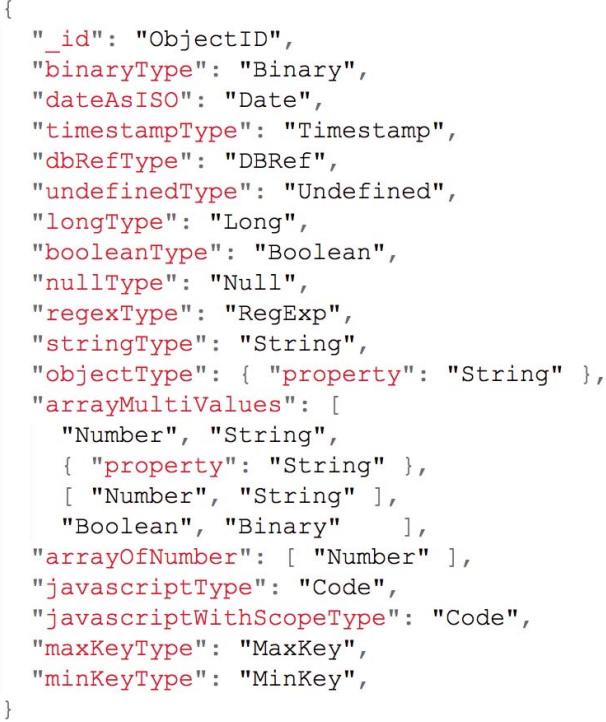
\includegraphics[width=0.6\linewidth]{figures/rawschema.png}
  \vspace{-10pt} % Adjust the value (e.g., 10pt) to your desired spacing
  \caption{Raw Schema \cite{frozza2018approach}}
  \label{fig:rawschema}
\end{figure}

\begin{table}[ht]
  \centering
  \caption{Comparison With Wang et al \cite{wang2015schema}}
  \vspace{-10pt}
  \label{tab:example}
  \resizebox{0.4\textwidth}{!}{
    \begin{tabular}{|c|c|c|c|c|}
      \hline
      \multicolumn{2}{|c|}{Datasets} & \multicolumn{2}{|c|}{JSON Schema Discovery} & \multicolumn{1}{|c|}{Wang et al \cite{wang2015schema}} \\
      \hline
      Collection & N\char`_JSON & RS & ROrd & FS\\
      \hline
      drugs & 3662 & 2818 & 2818 & 2818 \\
      \hline
      companies & 24367 & 21312 & 21312 & 21302 \\
      \hline
      movies & 30330 & 25140 & 25140 & 25137 \\
      \hline
    \end{tabular}
  }
  \smallskip
  \vspace{1pt}
  \parbox{0.4\textwidth}{%
    \centering
    \raggedright
    \footnotesize
    N\_SON - Number of JSON documents. RS - Raw schemas.\newline ROrd - Raw schemas with ordered structure. TB - Time to obtain the raw schemas. TT - Total time.
  }
        \label{table1}

\end{table}

\subsection{Successful Confirmation of Results}

Based on the provided experimental setup and expected outcomes, successfully obtaining identical numbers for N\_JSON, RS, and ROrD in Table~\ref{table1} will confirm the validity and reproducibility of the results, aligning with the findings of Frozza et al. ~\cite{frozza2018approach}. Additionally, we will employ hash verification methods. This will involve calculating the hash values of the generated data from our experiment using various cryptographic hash functions such as MD5, SHA-1, or SHA-256, and comparing them to the hash values of the data in Table~\ref{table1}. Moreover, to facilitate a basic structural consistency check between JSON files, a simple script can be implemented to assess whether the files share identical values at the top level, ensuring a fundamental validation of the data structure’s integrity.


\newpage


\section{Reproduction efforts}

In the subsequent section, we delineate the endeavors employed to replicate the findings documented by Frozza et al. \cite{frozza2018approach} as depicted in Table\ref{table1}. This includes elucidating the reproduction procedure, wherein we utilize the identical tool and dataset employed in the original study. Furthermore, we present the results and compare them with the original experiment's findings, affirming the successful reproduction thereof, and discuss potential threats to the validity of the experiment's conclusions.


\subsection{Reproduction Procedure}
The reproduction effort involved cloning the JSON Schema Discovery\footnote{https://github.com/feekosta/JSONSchemaDiscovery} application, along with the \textit{companies}, \textit{movies}, and \textit{drugs\footnote{https://github.com/feekosta/datasets}} datasets, as utilized in the original experiment by Frozza et al. ~\cite{frozza2018approach}. We proceeded by inserting the datasets into a MongoDB database. Subsequently, we executed the JSON Schema Discovery tool on the datasets, generating schemas. 

Upon conducting the experiment, the results obtained were compared with those reported in the original experiment conducted by Frozza et al. ~\cite{frozza2018approach}. The results are presented in Table~\ref{table2}, where "RepEng" denotes the results from our experiment.

\input{dynamicTable}
\vspace{-5pt}
Comparing the results of our experiment with those of Frozza et al. ~\cite{frozza2018approach}, it is evident that the reproduced outcomes exactly match. Since we obtained identical figures for N\_JSON (Number of JSON documents), RS (Raw schemas), and ROrD (Raw schema with ordered structure), we can confidently conclude that our reproduction was successful.

\subsection{Limitations and Threats to Validity}

Despite successfully reproducing the same number of files, it is crucial to acknowledge certain limitations and potential threats to the validity of the data. A significant concern arises from the unavailability of the content of schemas generated by Frozza et al. \cite{frozza2018approach}. For instance, Table~\ref{table1} indicates the generation of 2818 raw schemas for the collection of drugs; however, without access to the content of these schemas, our ability to conduct thorough comparisons and validations is hindered. This lack of access prevents us from performing hash verification methods, as we are unable to compare the hash values of our generated data with the hash values of the generated files by Frozza et al. \cite{frozza2018approach}. The absence of access to the schema content also inhibits the execution of our script designed for basic structural consistency checks between JSON files.

Considering the use of the same tool and dataset as the original experiment, we assess this limitation as minor, as it likely maintains consistency in content generation.
 

\subsection{Summary}
Frozza et al. \cite{frozza2018approach} propose a JSON Schema Discovery approach to address challenges in NoSQL databases' schemaless JSON documents. Their approach generates unified schemas from JSON data, aiding in data management. We aimed to independently obtain the same result using the authors' own artifact. Our results, detailed in Table~\ref{table2}, match theirs precisely, confirming our successful reproduction effort. However, the unavailability of schema content limits our ability to thoroughly compare the results' content.


\bibliographystyle{ACM-Reference-Format}
\bibliography{sample}

\end{document}
\endinput